Wir betrachten hier einige Testfunktionen, die als Zielfunktion
verschiedener restringierter Optimierungsaufgaben benutzt werden k�nnen.

\begin{testfunction}
Quadratische Funktion in $\R^n$
\[
  f(x) := \| x - d \|^2 = \sum_{k=1}^{n} (x_k - d_k)^2
\]
\end{testfunction}
Die erste Testfunktion ist eine einfache mehrdimensionale Parabel
mit Minimalstelle im Punkt~$d$ und Optimalwert~0.

\begin{testfunction}
Exponentielle Funktion
\[
  f(x) := e^{\|x\|^2} = e^{\sum_{k=1}^{n} x_k^2}
\]
\end{testfunction}
\begin{figure}[ht]
  \centering
  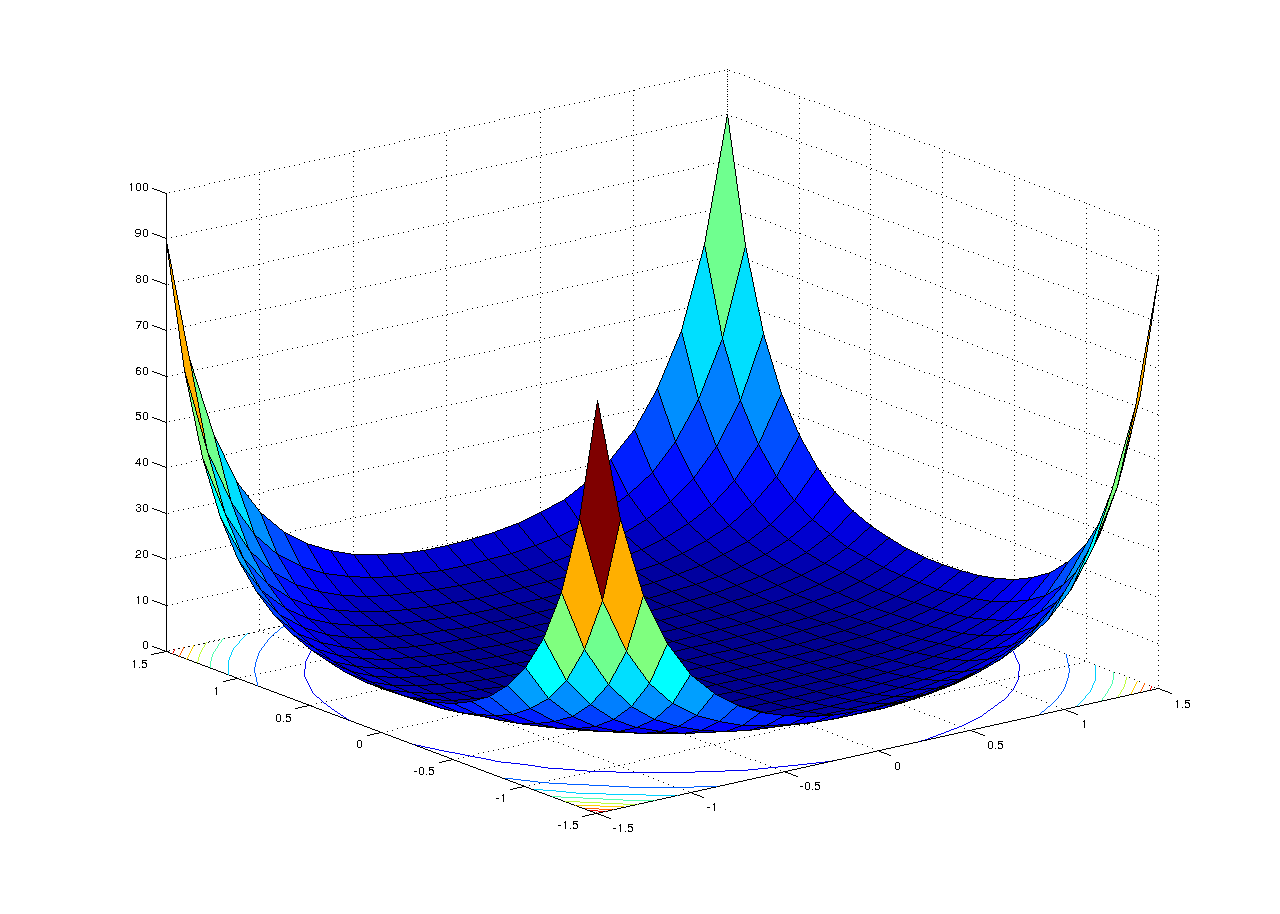
\includegraphics[width=0.75\textwidth]{exp-func}
  \caption{Exponentielle Funktion}
  \label{fig:exp_func}
\end{figure}
Die zweite Testfunktion ist eine exponentielle Funktion
mit Minimalstelle im Ursprung und Optimalwert~1.
Diese Funktion ist herausfordend, weil ihre Funktionswerte sehr schnell
gro� werden k�nnen.

\begin{testfunction}
Rosenbrock-Funktion
\[
  f(x) := 100(x_2-x_1^2)^2+(1-x_1)^2
\]
\end{testfunction}
\begin{figure}[ht]
  \centering
  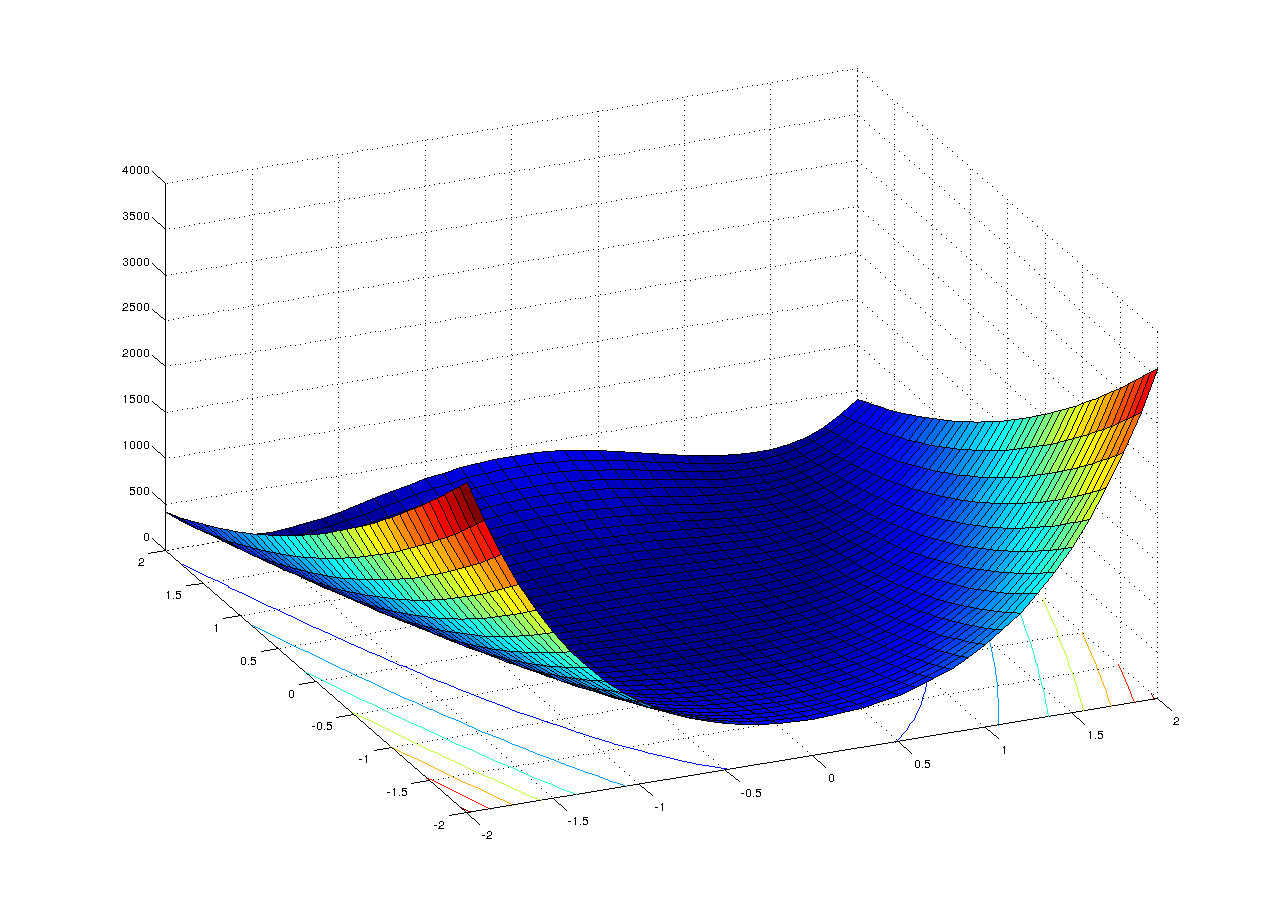
\includegraphics[width=0.75\textwidth]{rosenbrock}
  \caption{Rosenbrock-Funktion}
  \label{fig:rosenbrock}
\end{figure}
Die Rosenbrock-Funktion hat ein einziges Minimum
an der Stelle $\xopt = (1,1)^T$ mit $f(\xopt) = 0$.
Diese Funktion ist nicht einfach zu l�sen, da
das Minimum in einem schmalen "`bananenf�rmig"' gekr�mmten Tal liegt.
Als Anfangspunkt wird normalerweise den Punkt $x^0 = (-1,1)^T$ genommen.

\begin{testfunction}
Himmelblau-Funktion
\[
(x_1^2+x_2-11)^2 + (x_1+x_2^2-7)^2
\]
\end{testfunction}
\begin{figure}[ht]
  \centering
  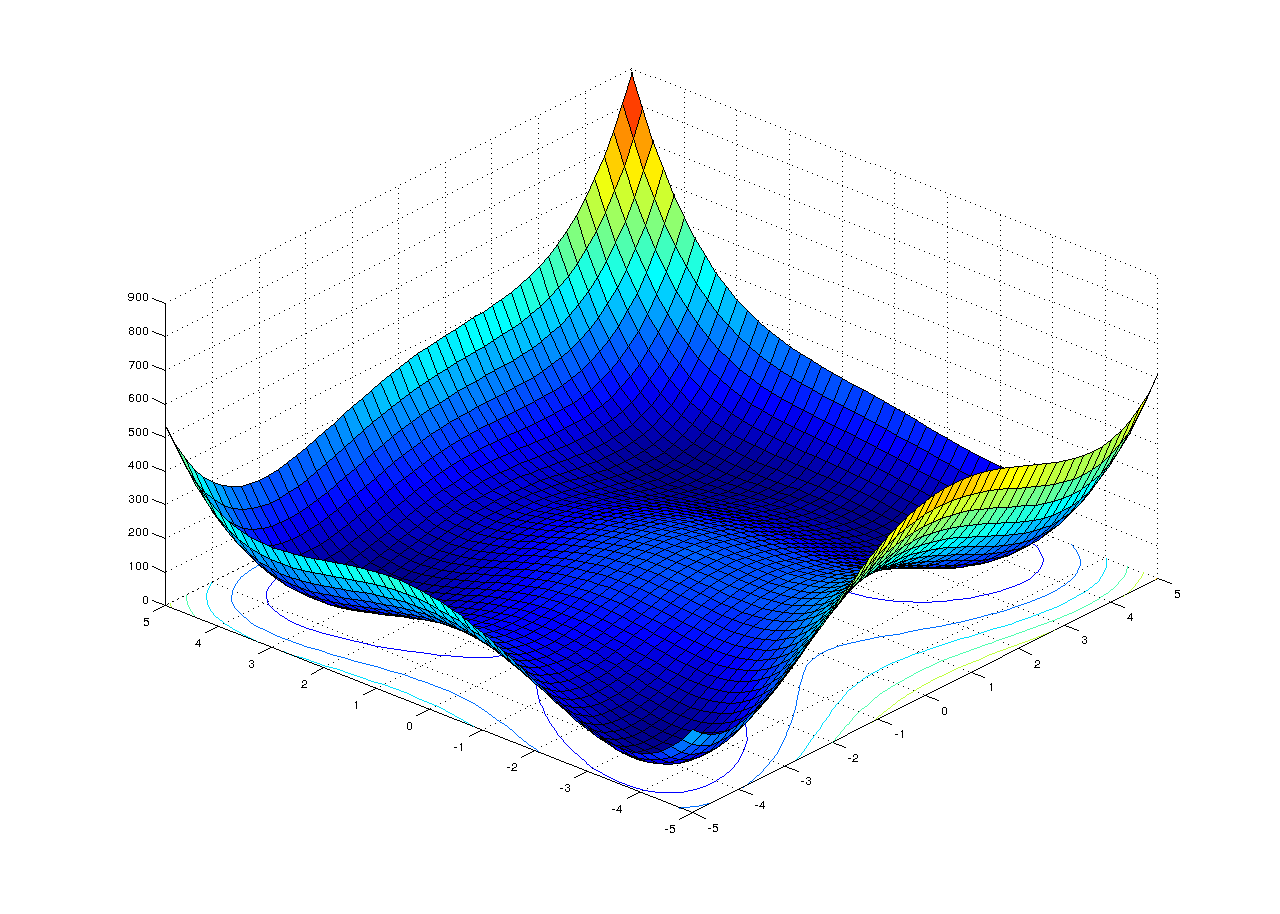
\includegraphics[width=0.75\textwidth]{himmelblau}
  \caption{Himmelblau-Funktion}
  \label{fig:himmelblau}
\end{figure}
Die Himmelblau-Funktion ist ein Polynom 4.~Grades
mit vier globale Minimalstellen.
Der Optimalwert ist 0.

\begin{testfunction}
Bazaraa-Shetty-Funktion
\[
  f(x) := (x_1-2)^4+(x_1-2x_2)^2
\]
\end{testfunction}
\begin{figure}[ht]
  \centering
  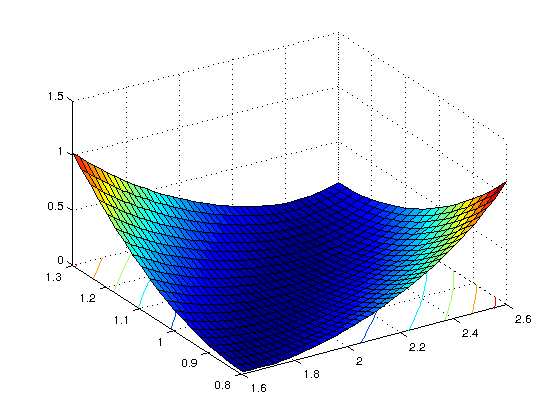
\includegraphics[width=0.75\textwidth]{bazaraa-shetty}
  \caption{Bazaraa-Shetty-Funktion}
  \label{fig:bazaraa_shetty}
\end{figure}
Die Bazaraa-Shetty Funktion ist ein Polynom 4.~Grades
mit einem globalen Minimum in $\xopt = (2,1)^T$
und Optimalwert 0.

\begin{testfunction}
Schuldt Funktion
\[
x_2+10^{-5}(x_2-x_1^2)^2
\]
\end{testfunction}

\begin{testfunction}
Asaadi Funktion
\[
x_2+\frac{1}{3}(x_1+1)^3
\]
\end{testfunction}

\begin{testfunction}
McCormick Funktion
\[
\sin(x_1+x_2) + (x_1-x_2)^2 - 1.5x_1 + 2.5x_2 + 1
\]
\end{testfunction}

\begin{testfunction}
Dixon Funktion
\[
(1-x_1)^2 + \sum_{k=1}^{9} (x_k^2-x_{k+1})^2 + (1-x_{10})^2
\]
\end{testfunction}

\begin{testfunction}
Colville Funktion
\begin{multline}
  f(x) := 100(x_2-x_1^2)^2 + (1-x_1)^2 + 90(x_4-x_3^2)^2 + (1-x_3)^2 \\
    + 10.1((x_2-1)^2 + (x_4-1)^2) + 19.8(x_2-1)(x_4-1) \notag
\end{multline}
\end{testfunction}

\begin{testfunction}
Betts Funktion
\[
2 - \frac{1}{2}x_1x_2
\]
\end{testfunction}

\begin{testfunction}
Paviani Funktion
\[
  f(x) := - (\ln(x_1-2))^2 - (\ln(10-x_1))^2
            - (\ln(x_2-2))^2 - (\ln(10-x_2))^2
\]
\end{testfunction}
